\chapter{Test}
In this chapter, we go through the tests, which got made during the development of the Ezuino programming language. At the beginning of the project, the only tests which could be done were using the language made by the ANTLR grammar file and testing different dummy programs, and test whenever ANLTR report any ambiguity or syntax error within the code entered. Multiple programs got written, to ensure that we got around every syntax and scenario possible, to avoid any future error, once we’ve started building the Concrete Syntax Tree (CST) and the Abstract Syntax Tree (AST).  One of the programs can be reviewed in figure \ref{test0} and \ref{test00}.

\begin{figure}[H]
\centering
\frame{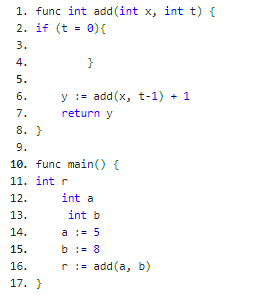
\includegraphics[scale=1]{figures/test/test0.png}}
\caption{Test}
\label{test00}
\end{figure}

\begin{figure}[H]
\centering
\frame{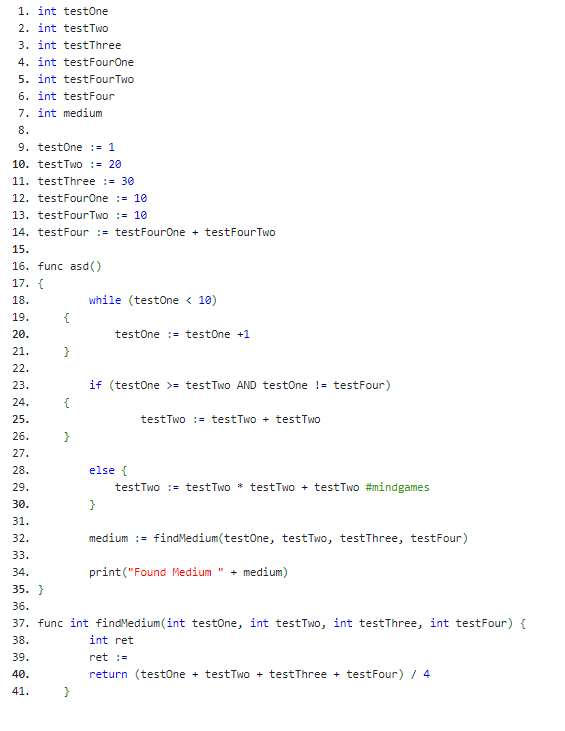
\includegraphics[scale=1]{figures/test/test6.png}}
\caption{Test}
\label{test0}
\end{figure}

\section{JUnit Testing}
Once the development of the compiler in Java has started, JUnit testing has been used during the remaining of the process. This section will go through some of the JUnit test, which gets written during the development process. The tests have been categorized into three sections: CST, AST, and Lexer/Parser test. 
Starting from the beginning of development, we get to look at the Lexer/Parser test, which is the classes ANTLR 4 has generated and using the ANTLR maven package, can use. In these test classes, we use the Error Handler, which was explained the chapter 6, to check whenever there is an error, during the lexing/parsing of a small code snippet. If the error handler finds an error, depending on the asset, the test will either fail or pass. 
\begin{figure}[H]
\centering
\frame{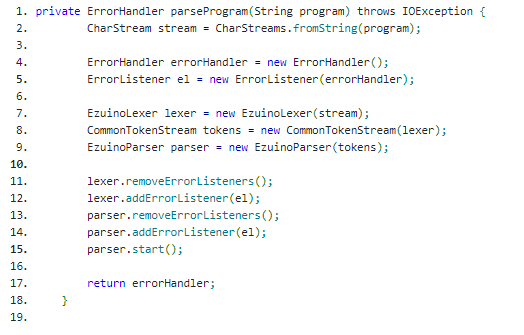
\includegraphics[scale=1]{figures/test/test2.png}}
\caption{Test}
\label{test1}
\end{figure}
Figure \ref{test1} shows a method, which is used to initialize the error handler, lexer and parser with the code, as inputted by a string. 
\begin{figure}[H]
\centering
\frame{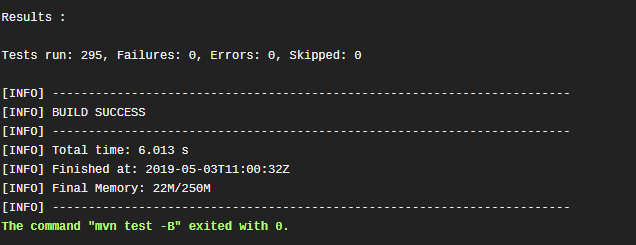
\includegraphics[scale=1]{figures/test/test4.png}}
\caption{Test}
\label{test2}
\end{figure}
On figure \ref{test2}, we have the first test, which a simple integer declaration, where we declare the variable a. We assert that the errorhandler should’t have any errors, as this is the correct syntax in this case – using the hasErrors() method, which is a part of the error handler class, and will return an Boolean value. 
Moving on towards the type checker and CST tests, test on figure 4 shows a test with a multiplicative expression: 
\begin{figure}[H]
\centering
\frame{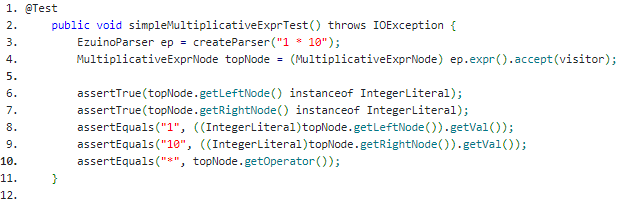
\includegraphics[scale=0.86]{figures/test/test5.png}}
\caption{Test}
\label{test3}
\end{figure}
Figure \ref{test3} shows the test of the expression (1 * 10), where we test if both the right and left side nodes of the MultiplicativeExprNode is of type Integers. If they aren’t, we can already throw an exception. Next, we’re checking if the values of the left and right node are the ones which we’ve entered in our expression. In this case, we assert that the left node has the value 1, and the right node has the value 10.  We also check that the operator in this expression is a multiplicative operator.
The code generation tests for Java bytecode and C, has been tested by taking the Ezuino program, and comparing it to an expected output of the C programming language. If the output is correct, the tests are successful.  
\section{Continuous Integration}
During the development of the programming language, more tests has been added in the development process. The final number of tests, is around 250+, in multiple classes. This is a significant number of tests to run each time an AST or node has been changed, so Continuous Integration (CI), has been deployed, to automate each test and compile the software after each Git Commit (GC) or Pull Request (PR).  The CI used for this purpose was Travis CI, which is a free CI service for public git repositories. \\
\begin{figure}[H]
\centering
\frame{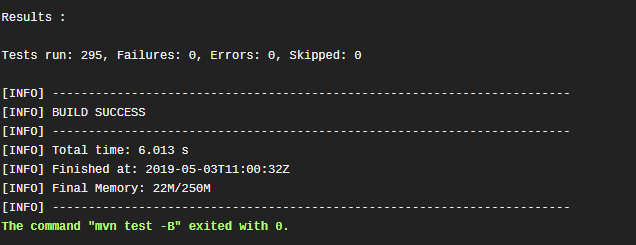
\includegraphics[scale=0.8]{figures/test/test1.png}}
\caption{Test}
\label{testa}
\end{figure}
On figure \ref{testa}, a Travis build has run on a GC, which has recently been committed. In this result, we can see that the 295 tests have been ran successfully, and the program ran without any error. In case the program finds an issue, and add it to the Error Handler, it will fail the build, but no the tests. Also, the other way around, if a node has been changed, but the program may build, if one tests fails, the Travis check will fail as well. \\
\\
This chapter has been going through a few of the around 300 tests made in this project, and given an insight in the tests process which has been made during the development of the Ezuino programming language. It is very essential to avoid errors in the compiler in a programming language, so testing of features has been prioritized, however, there are still testing forms like code coverage and whitebox (branch testing), which has not been done at this time. If the Ezuino programming language were to get a commercial release, these tests are essential to provide a large sum of error or failure correction, as a programming language is very abstract. 
